% !TeX root = ../../../book.tex

\subsection{其他计数对象}

\subsubsection*{$[k]$ 中的 $n$-元组}

扑克牌是一种很好且标准的物理计数对象。大多数人对扑克牌都很熟悉,因为每张牌都有两个属性——花色和点数——这使得我们能够设计出许多有趣的组合问题。一个更``抽象''的标准计数对象是具有指定长度的自然数列表。为此,我们引入以下定义,以便能够简洁地引用这些集合。

\begin{definition}
    给定 $n,k \in \mathbb{N}$,则
    \[T_{k,n} = [k]^n = \{(a_1, a_2, \dots , a_n) \mid \forall i \centerdot a_i \in [k]\}\]
    也就是说,$T_{k,n}$ 是所有元素属于 $[k]$ 的 $n$-元组的集合。
\end{definition}

注意:我们选用字母 $T$ 是因为这些对象是 \emph{$n$-元组 (Tuple)},即长度为 $n$ 的有序列表。值得一提的是,当 $k$ 是一个较小的数(如 $2$ 或 $3$)时,通常会将集合 $[k]$ 替换为 $[k - 1] \cup \{0\}$。例如,二进制 $n$ 元组在数学中非常常见,部分原因在于它在计算机科学中的广泛应用。因此,当 $k = 2$ 时,我们常常考虑元素取自集合 $\{0, 1\}$,而非 $\{1, 2\}$,且长度为 $n$ 的有序列表。由于我们关注的是这些集合的组合性质(例如``具有属性 $P$ 的序列有多少?''),实际上选择哪种约定并不重要。事实上,通过在基本集合 $[k]$ 与 $[k - 1] \cup \{0\}$ 之间建立双射,可以轻松证明:
\[|T_{k,n}| = |[k]^n| = k^n = |([k - 1] \cup \{0\})^n|\]
这部分证明留给你来完成$\smiley{}$

在下一节中,我们将看到许多计数论证可以通过选取合适的 $k$ 和 $n$,并考虑有序列表的附加属性来简洁表达。现在,让我们看几个简单的例子并探讨一些应用。在每个例子中,我们将研究子集 $S \subseteq T_{k,n}$,其中元素具有某些特定性质;具体来说,我们将通过计算 $S$ 中元素的个数来得到 $|S|$。我们从一些非常简单的例子开始,然后逐步深入更加复杂的案例。本节末尾的练习将进一步拓展这些概念。

\begin{example}
    设 $n=4, k=3$

    \begin{enumerate}[label=(\arabic*)]
        \item $|T_{3,4}|$ 是多少?\\
              要计算 $T_{3,4}$ 的元素数量,我们可以通过一个四步过程来构建这个集合,其中第 $i$ 步对应于选择 $4$-元组中的第 $i$ 个元素。在每一步中,我们有 $3$ 个选项(每个元素来自 $\{1, 2, 3\}$),因此根据乘法原理,$T_{3,4}$ 共有 $3 \cdot 3 \cdot 3 \cdot 3 = 3^4 = 81$ 个元素。(注意:请参见练习 \ref{},其中要求证明 $|T_{n,k}| = n^k$ 的一般情况。)
        \item $T_{3,4}$ 中有多少个元素不包含数字 \verb|1|?\\
              要计算 $T_{3,4}$ 中不包含 \verb|1| 的元素数量,我们可以通过限制每一步的选项来简化四步过程。具体来说,$T_{3,4}$ 中不包含 \verb|1| 的元素,其 $4$ 个位置只能从集合 $\{2, 3\}$ 中选择。因此,根据乘法原理,有 $2 \cdot 2 \cdot 2 \cdot 2 = 2^4 = 16$ 个这样的元素。
        \item $T_{3,4}$ 中有多少个元素恰好包含一个 \verb|1|?有多少个恰好包含两个 \verb|1|?有多少个恰好包含三个 \verb|1|?有多少个恰好包含四个 \verb|1|?\\
              如何计算 $T_{3,4}$ 中恰好含有一个 \verb|1| 的元素数量?是否可以使用与上一问相同的思路?答案是不完全适用!在这个过程中,每一步的可选项数量可能会发生变化,这取决于是否已经在 $4$-元组中放置了一个 \verb|1|。因此,我们需要一种新方法。我们可以考虑先在 $4$-元组中的某个位置放置一个 \verb|1|,然后用 $\{2, 3\}$ 中的元素填充剩余位置。具体来说,我们可以通过以下四个步骤构建恰好含有一个 \verb|1| 的 $4$-元组:
              \begin{enumerate}[label=(\alph*)]
                  \item 选择四个位置中的一个放置来数字 \verb|1|:有 ${4 \choose 1}=4$ 种方法。\\
                        然后,对于剩下的三个位置,从左到右依次填入 $\{2, 3\}$ 中的元素。
                  \item 对于第一个剩余位置,从 $\{2, 3\}$ 中选择一个元素:有 $2$ 种方法。
                  \item 对于第二个剩余位置,从 $\{2, 3\}$ 中选择一个元素:有 $2$ 种方法。
                  \item 对于第三个剩余位置,从 $\{2, 3\}$ 中选择一个元素:有 $2$ 种方法。
              \end{enumerate}
              因此,$T_{3,4}$ 中共有 $4 \cdot 2^3 = 32$ 个这样的元素。
    \end{enumerate}

    或许上述论证略显繁琐。实际上,我们可以简化为两个步骤:首先选择 \verb|1| 的位置,然后从 $\{2, 3\}$ 中为剩余位置选择值。这只是表述上的差异,其本质相同。我们提供这些额外细节是为了帮助你理解论证的基本原理,从而你能将这些思路应用于自己的证明。

    或许我们在这个论证中显得有些啰嗦。其实可以简化为两个步骤:首先确定 \verb|1| 的位置,然后从 $\{2, 3\}$ 中选择余下 $3$ 个位置的值。这只是表述上的不同,本质上证明的是同一事实。我们提供这些额外的细节是为了确保你能理解我们的论证和其中的基本原理,这将帮助你将这些思路应用到你自己的证明中。

    我们可以用类似的方法计算 $T_{3,4}$ 中恰好有两个 $1$ 的元素数量。唯一的区别在于步骤 1:我们需要从 $4$ 个位置中选择 $2$ 个位置来放置 \verb|1|,这有 ${4 \choose 2}$ 种选择方法。然后,剩余两个位置需要从 $\{2, 3\}$ 中选择元素。因此,$T_{3,4}$ 中有
    \[{4 \choose 2} \cdot 2^2 = 24\]
    个这样的元素。

    我们留给你来验证 $T_{3,4}$ 中恰好有三个 \verb|1| 的元素有 $8$ 个,恰好有四个 \verb|1| 的元素有 $1$ 个。我们也留给你来验证并解释为什么 $16 + 32 + 24 + 8 + 1 = 81$ 是合理的。(挑战性问题:你能将这个结果推广到任意 $n$ 和 $k$ 吗?)
\end{example}

\begin{example}
    设 $n \ge 3$。我们来计算以下几种二进制 $n$-元组的数量:
    \begin{enumerate}[label=(\alph*)]
        \item 恰好有三个 \verb|1|;
        \item 至少有三个 \verb|1|;
        \item 包含偶数个 \verb|1|。
    \end{enumerate}

    我们这里讨论的集合是 $\{0, 1\}^n$,即所有由 \verb|0| 和 \verb|1| 构成的 $n$-元组。(注意,这并不是前面定义的集合 $T_{2,n}$,但我们已经解释了如何在这两个集合之间建立双射。)

    对于问题 (a),我们采用与前例相同的方法:首先从 $n$ 个位置中选择 $3$ 个位置放置 $1$,然后用 \verb|0| 填充剩余的 $n-3$ 个位置。第一步有 ${n \choose 3}$ 种选择方式,第二步是确定的(即只有一种方式),因此共有 ${n \choose 3}$ 个二进制 $n$-元组恰好有三个 \verb|1|。(注意:我们规定 $n \ge 3$ 是为了确保答案非零。当 $n \le 2$ 时,显然不存在这样的元组!这也验证了当 $\ell > n$ 时,${n \choose \ell} = 0$。)

    对于问题 (b),我们沿用问题 (a) 的方法,但将其推广到任意自然数 $\ell$。具体来说,计算恰好有 $\ell$ 个 \verb|1| 的二进制 $n$-元组数量时,先选择 $n$ 个位置中的 $\ell$ 个填入 \verb|1|,其余位置填入 \verb|0|。为了得到至少三个 \verb|1|,我们需要考虑恰好有三个、四个……直至 $n$ 个 \verb|1| 的情况。更严格地说,对每个满足 $3 \le \ell \le n$ 的 $\ell$,设 $A_\ell$ 为恰好有 $\ell$ 个 \verb|1| 的二进制 $n$-元组集合。每个至少有三个 \verb|1| 的二进制 $n$-元组都恰好属于一个 $A_\ell$。因此,这些集合构成了一个\emph{划分},每个部分对应特定数量的 \verb|1|。根据加法原理,总数为
    \[\sum_{\ell = 3}^{n} |A_\ell| = \sum_{\ell = 3}^{n} {n \choose \ell}\]
    
    你可能会问,以求和形式表示的答案是否\emph{可接受}?从某种意义上看,它是可接受的;就在十分钟前,我们还不知道至少有三个 \verb|1| 的二进制 $n$-元组的数量,而现在我们有了更清晰的认识。然而,上述解法更偏向于一种计算精确数值的方法。假如有人在街上问你:``快!告诉我至少有三个 \verb|1| 的二进制 $n$-元组的数量!''你会怎么回答?你可能会说:``等等,我需要逐项计算再求和……''这显然不够理想,对吧?如果有一个形式简单的解会更方便;例如,将它写成一个二项式系数,或者少数几个二项式系数的和、差、积或商。这样,无论 $n$ 多大,我们都能通过固定数量的简单步骤高效计算出答案,且步骤数不随 $n$ 的增大而增加。而上面求和公式的项数会随 $n$ 的增大而增大,这并不理想。

    我们将细节的验证和解释留给你,但我们断言:通过应用加法原理,可以对所有二进制 $n$-元进行适当划分,从而证明
    \[2^n = {n \choose 0} + {n \choose 1} + {n \choose 2} + \sum_{\ell = 3}^{n} {n \choose \ell}\]
    实际上,该等式的证明涉及后续章节的技术,但我们相信你能理解其中各项的含义及其成立的原因。重要的是,通过重新整理该等式,我们得到一个形式上更优的解:
    \[\sum_{\ell = 3}^{n} {n \choose \ell} = 2^n - {n \choose 0} - {n \choose 1} - {n \choose 2}\]
    看看我们的成果!无论 $n$ 多大,我们只需计算四项。这里\emph{固定项数}是关键。事实上,我们非常喜欢这种形式的解,因此称它为\textbf{闭合解}。其特点是无需``多余''的求和,项数固定,不随变量值变化。

    通常,在解决组合数学问题时,我们总是力求寻找\textbf{闭合解}。有时,我们容易得到非闭合形式的解(有人称之为``开放解''),但将其转化为闭合形式可能需要巧妙思考。在本例中,我们观察到所有二进制 $n$-元组可按 \verb|1| 的个数分为零个、一个、两个或至少三个。这种闭合解不仅能更快、更简便地计算表达式,还能提供对问题底层结构的更多见解。因此,我们始终追求闭合解。

    现在,别忘了问题 (c)!我们采用与 (b) 类似的技术,将具有偶数个 \verb|1| 的二进制 $n$-元组划分为恰好有零个 \verb|1|(记住,$0$ 是偶数!)、两个 \verb|1|、四个 \verb|1|,等等。不过,必须注意上限,因为 $n$ 未必是偶数!回顾向下取整函数,它将实数向下舍入到不大于它的最大整数,例如 $\lfloor 5.7 \rfloor = 5$。考虑到这一点,我们断言具有偶数个 \verb|1| 的二进制 $n$-元组数量为
    \[\sum_{\ell=0}^{\lfloor n/2 \rfloor} {n \choose 2\ell}\]
    我们将解释该断言的机会留给你。试着向你的朋友证明并说服他们其正确性。不要放弃,直到他们完全信服!我们不再寻求其\emph{闭合解},因为这已超出当前范围……但请思考:你能从该求和中推断出什么?当 $n$ 为偶数时如何?当 $n$ 为奇数时又如何?是否存在类似求和与之关联?你能得出什么结论?
\end{example}

\begin{example}
    计算 \verb|1| 成对出现的二进制 $4$-元组的数量。例如,我们会把 $(1, 1, 0, 0)$ 和 $(1, 1, 1, 1)$ 算进来,但不会包括 $(1, 0, 1, 1)$ 或 $(0, 1, 1, 1)$。然后,我们将此方法扩展到二进制 $5$-元组,看看能否找到一个通用模式。

    如果一个 $4$-元组中的 \verb|1| 成对出现,则 \verb|1| 的总数只能是 $0$、$2$ 或 $4$。我们定义集合 $S_0$、$S_2$ 和 $S_4$,分别表示包含 $0$、$2$ 或 $4$ 个 \verb|1| 且 \verb|1| 成对出现的二进制 $4$-元组。(注意:$S_2$ 并非指仅有两个 $1$ 的二进制字符串,否则会错误地包含像 $(1, 0, 1, 0)$ 这样的字符串。)这些集合构成了所有符合条件的二进制 $4$-元组的一个划分,因此我们只需计算各集合的元素数量,再应用加法原理求和即可。
    \begin{itemize}
        \item 为了计算 $|S_0|$,我们需要计数没有 $1$ 的二进制 $4$-元组,这样的 $4$-元组显然只有一个:$(0, 0, 0, 0)$。
        \item 为了计算 $|S_2|$,我们需要计数有两个连续 $1$ 且其余位置为 $0$ 的二进制 $4$-元组。手动枚举所有情况,
              \[(1, 1, 0, 0) \qquad (0, 1, 1, 0) \qquad (0, 0, 1, 1)\]
              显然,这样的元组只有 $3$ 个。(你能给出一个更巧妙的论证来说明为什么只有 $3$ 个吗?在研究 $5$-元组时,我们会回到这个问题。)
        \item 为了计算 $|S_4|$,我们需要计数有四个 $1$ 的二进制 $4$-元组。显然 $(1, 1, 1, 1)$ 是唯一的答案。
    \end{itemize}
    根据加法原理,共有 $1 + 3 + 1 = 5$ 个 $1$ 成对出现的二进制 $4$-元组。

    要回答关于 $5$-元组的问题,需要更巧妙的方法。我们类似地定义集合 $S_0$、$S_2$ 和 $S_4$,但将 $4$-元组变为 $5$-元组。这三个集合仍构成所有符合条件的二进制 $5$-元组的一个划分。只需计算各集合的元素数量,再应用加法原理求和即可。
    \begin{itemize}
        \item $|S_0|=1$,因为只有一个不含 $1$ 的 $5$-元组:$(0, 0, 0, 0, 0)$。
        \item 为了计算 $|S_2|$,我们可以手动枚举所有情况,但最好能提出一个适用于任意 $k$-元组(其中 $k \in \mathbb{N}$)的通用方法。要有一对连续的 $1$ 且其余位置为 $0$,我们可以将``$1, 1$''视为一个整体,放置在三个 $0$ 之间。因此,我们实际上是在计算如何将一个特殊整体放置到长度为 $4$ 的有序列表中,然后用另一个固定元素确定性地填充剩余位置。当然,有 $4$ 种方法可以做到这一点,手动写出这些情况可以验证这一点。(实际上我们注意到,一对连续的 $1$ 可由元组中\emph{第一个} $1$ 的索引确定;该索引可以是 $\{1, 2, 3, 4\}$ 中的任意一个,所以有 ${4 \choose 1} = 4$ 种选择。)
        \item 上面的方法同样适用于 $|S_4|$ 的情况。这种情况下,我们有两对连续的 $1$,因此可以将每对``$1,1$''看作一个整体。这样,我们实际上有两个``$1,1$''和一个 $0$ 需要放入长度为 $3$ 的有序列表中。由于两个``$1,1$''是相同的,我们可以通过选择这两个``$1,1$''的位置来计算有序列表的数量。因此,有 ${3 \choose 2} = 3$ 种排列方式。(同样,我们也可以通过选择 $0$ 的位置来计算,即 ${3 \choose 1} = 3$ 种选择。)
    \end{itemize}
    因此,共有 $1 + 4 + 3 = 8$ 个 $1$ 成对出现的二进制 $5$-元组。
\end{example}

\subsubsection*{字母表与单词}

从 $[n]$ 中选取元素组成 $k$-元组的概念与从给定\emph{字母表}中构造\emph{单词}的概念非常相似。实际上,从数学的角度讲,这两个概念是\emph{等价的},并没有引入新的内容。不过,这种表述可以采用不同的术语,并且与一些``现实世界''的概念和问题相关联。出于这一原因,同时考虑到某些表述可能更易于理解,我们在本小节中介绍这一观点,并与前一小节的内容建立联系。

我们将通过若干例子来阐述本小节的核心思想。在每个例子中,会给定一个字母表,其元素是用于构造单词的字母。但需要注意的是,这里的``单词''实际上是指从给定字母表中选取的任何有序字符串。例如,在第一个例子中,我们使用标准英文字母表;此时,\verb|ZPQ| 是一个完全有效的三字母单词(尽管发音可能有些困难!)。我们采用这种泛化定义的主要原因是为了避免语义或词源上的争议,例如争论 \verb|REALISE| 是否是 \verb|REALIZE| 的可接受变体,或者 \verb|ZZZ| 是否应被视为拟声词。这意味着我们需要剥离``单词''一词的部分内涵,仅将其视为由字母组成的字符串,除了字母及其顺序外,不具其他固有意义。

\begin{example}
    让我们以标准的 $26$ 个英文字母为例。
    \begin{enumerate}
        \item 用这个字母表可以组成多少个 $3$ 字母单词?\\
              这等价于求 $T_{26,3}$ 的大小。我们有 $26$ 个字母,要组成长度为 $3$ 的有序列表。通过建立集合 $\{A, B, C, \dots, Z\}$ 和 $[26]$ 之间的双射(类似于你小时候可能玩过的替换密码),我们可以严格证明这个问题等价于求 $|T_{26,3}|$。\\

              即便不建立这种联系,我们也可以观察到构造一个 $3$ 字母单词是一个 $3$ 步过程(从左到右填入字母),每一步有 $26$ 种选择,从而轻松计算出 $3$ 字母单词的数量。因此,有 $26^3$ 个 $3$ 字母单词。
        \item 可以组成多少个 $4$ 字母单词?\\
              根据同样的逻辑,有 $26^4$ 个 $4$ 字母单词。
        \item 可以组成多少个 $n$ 字母单词?\\
              这个问题留给你来解答。$\smiley{}$
        \item 有多少个以元音开头的 $4$ 字母单词?\\
              注意:我们将 $\{A, E, I, O, U\}$ 视为元音(尽管字母歌中可能将 $Y$ 也视为元音,但这里不包括 $Y$)。基于此,我们可以调整构造 $4$ 字母单词的过程,确保第一个位置是元音。第一步有 $5$ 种选择,后续三步每步有 $26$ 种选择。因此,有 $5 \cdot 26^3$ 个以元音开头的 $4$ 字母单词。
        \item 有多少个最多有 $2$ 个辅音的 $4$ 字母单词?\\
              辅音是非元音字母,因此根据定义,字母表中有 $21$ 个辅音。最多有两个辅音意味着恰好有 $0$ 个、$1$ 个或 $2$ 个辅音。因此,我们可以将单词划分为三个集合 $S_0$、$S_1$ 和 $S_2$,并分别计算它们的数量。应用乘法法则,可得:
              \begin{align*}
                  |S_0| & = 5^4                                  \\
                  |S_1| & = { 4 \choose 1 } \cdot 21 \cdot 5^3   \\
                  |S_2| & = { 4 \choose 2 } \cdot 21^2 \cdot 5^2
              \end{align*}
              因此,最多有两个辅音的 $4$ 字母单词的数量为:
              \[5^4 +  4 \cdot 21 \cdot 5^3 + { 4\choose2 } \cdot 21^2 \cdot 5^2\]
              (挑战性问题:有多少个 $4$ 字母单词至少有三个辅音?利用这里的结论和 $26^4$ 给出答案。)\\

              关于 $S_2$ 的以下论点有什么问题:要构造一个恰好有两个辅音的 $4$ 字母单词,先选择两个辅音,然后为第一个辅音选择一个位置,再为第二个辅音选择一个位置,最后用元音填充剩余两个位置。因此,得到:
              \[{ 21 \choose 2 } \cdot 4 \cdot 3 \cdot 5^2\]
              个这样的单词。\\

              仔细思考这个问题。记住,这些``找出错误''问题不仅要求识别错误,还要解释错误原因及如何修正。
        \item 有多少个由 $4$ 个不同字母组成的 $4$ 字母单词?\\
              我们可以直接通过一个四步过程来回答这个问题:从左到右填写四个字母,每一步可选的字母数比上一步减少一个。因此,有
              \[26 \cdot 25 \cdot 24 \cdot 23\]
              个由四个不同字母组成的 $4$ 字母单词。\\

              这看起来是不是很熟悉?回顾我们定义\emph{排列}的方法。这正是排列的思路!从一个包含 $26$ 个元素的集合中,我们想构造一个长度为 $4$ 且不重复的有序列表,即从 $26$ 个元素中选取 $4$ 个进行排列。推导出的公式表明,这样的排列共有
              \[{ 26 \choose 4 } \cdot 4! = \frac{26!}{4! \cdot 22!} 4! = \frac{26!}{22!} = 26 \cdot 25 \cdot 24 \cdot 23\]
              这个例子说明:通过利用已定义的术语和公式,并将问题与这些概念关联,我们可以快速求解。
        \item 有多少 $4$ 字母单词恰好有一个字母重复两次?\\
              要构造这样的单词,我们需要确定哪个字母重复了两次,以及它的两个位置在哪里。此外,还需要确定单词中另外两个字母是什么。因此,可以分三步进行:
              \begin{enumerate}[label=(\arabic*)]
                  \item 选择重复的字母;
                  \item 在四个位置中选择两个放置该字母;
                  \item 从剩下的 $25$ 个字母中选择两个放入剩余位置。
              \end{enumerate}
              因此,恰好有一个字母重复两次的 $4$ 字母单词的数量为
              \[{ 26 \choose 1 }{ 4 \choose 2 }{ 25 \choose 2 } \cdot 2!\]
        \item 有多少 $5$ 字母单词恰好有两个字母各自重复两次?\\
              按照类似逻辑,我们可以进行以下步骤:
              \begin{enumerate}[label=(\arabic*)]
                  \item 选择两个重复的字母;
                  \item 从 $5$ 个位置中选择两个放置第一个(按字母顺序)重复字母;
                  \item 从剩余 $3$ 个位置中选择两个放置第二个重复字母;
                  \item 从剩下的 $24$ 个字母中选择一个填充最后一个位置。
              \end{enumerate}
              因此,恰好有两个字母各自重复两次的 $5$ 字母单词的数量为
              \[{ 26 \choose 2 }{ 5 \choose 2 }{ 3 \choose 2 }{ 24 \choose 1 }\]
    \end{enumerate}
\end{example}
\clearpage
\begin{example}
    有多少种排列方式可以让字母 \verb|U| 与单词 \verb|ME| 在一起?$\smiley{}$

    你可能会想到用``排除法''来解决这个问题。也就是说,尝试计算所有不将字母 \verb|U| 置于单词 \verb|ME|(按此顺序)旁边的排列。你可以试试看会得到什么结果。然而,我们将提出一种不同的方法,并且认为这种方法更为简洁。该方法的思路在其他问题中同样适用,简而言之,就是将双字母单词 \verb|ME| 视为一个整体,如同单个字母一样处理。

    换个角度思考,与其询问从给定字母表中能组成多少种单词,不如探讨给定单词有多少种排列组合(即\emph{异序词})。考虑这些问题时必须小心,因为当字母重复时,情况会变得复杂。例如,单词 \verb|A| 有多少种异序词?单词 \verb|AAAAA| 呢?单词 \verb|AABBBCCCCDD| 呢?没错!你应该已经抓住了我们想要表达的核心观点。
\end{example}

\begin{example}
    让我们从一个简单的例子开始。单词 \verb|HEART| 有多少个异序词?记住,我们将字母的所有排列都视为有效单词,所以不要用拼字游戏的规则来思考这个问题 $\smiley{}$。(顺带一提,在拼字游戏中,这个问题的答案是 $4$ —— \verb|HEART, HATER, EARTH, RATHE|。)由于这个单词的每个字母都\emph{不同},答案很简单:只需计算 $5$ 个字母的全排列即可。因此,\verb|HEART| 有 $5! = 120$ 个异序词。

    \verb|APPLE| 有多少个异序词呢?注意到字母 \verb|P| 出现了两次,所以我们不能简单地考虑五个元素的全排列。如果那样做,每个单词实际上都会被重复计数两次;也就是说,\verb|APPLE| 这个单词会被重复计数。你能看出这两个单词有什么不同吗?我们只是交换了两个 \verb|P|!显然,它们是相同的单词,所以我们在考虑排列时需要把这一点考虑进去。

    我们该怎么处理这个问题呢?一个有用的技巧是给重复的 \verb|P| 打上``标签''。从左到右读取 \verb|APPLE|,我们称第一个 \verb|P| 为 $\mathtt{P_1}$,第二个 \verb|P| 为 $\mathtt{P_2}$。这将帮助我们理清重复的排列。现在,我们有五个不同的元素 —— $\mathtt{A, P_1, P_2, L, E}$ —— 所以我们可以考虑这些元素的所有 $5!$ 个排列。我们知道这样会导致重复计数,所以我们需要弄清楚重复计数的程度。定义 $G$ 为 \verb|APPLE| 的异序词集合(我们正在尝试计算 $|G|$),并定义 $M$ 为上述五个不同元素的全排列集合。$|G|$ 和 $|M|$ 之间有什么关系呢?

    要回答这个问题,我们可以考虑从 $G$ 的元素构造 $M$ 的元素。具体来说,我们可以通过先取 $G$ 的一个元素(\verb|APPLE| 的一个异序词),然后给 \verb|P| 打上标签来构造 $M$ 的一个元素。然而,这样并不能生成 $M$ 的所有元素。为此,我们必须从 $G$ 的每个元素中构造两个 $M$ 的元素;具体来说,我们需要给 \verb|P| 打上标签,然后考虑单词中 \verb|P| 的两种排列方式。让我们看一个例子:
    \begin{itemize}
        \item 取 $G$ 中的一个元素,例如 \verb|PAPEL|。
        \item 从左到右给 \verb|P| 打上标签:$\mathtt{P_1AP_2EL}$。
        \item 构建两种 \verb|P| 的排列,并将这两个词都作为 $M$ 的元素:$\mathtt{P_1AP_2EL} \in M$ 且 $\mathtt{P_2AP_1EL} \in M$。
    \end{itemize}
    由于两个 \verb|P| 有 $2! = 2$ 种排列方式,我们已经证明了 $|G| \cdot 2! = |M|$。我们描述了一个生成 $M$ 元素的两步过程并应用了乘法原理。因此,我们可以通过重新整理这个方程来得到我们要寻找的数量:
    \[|G| \cdot 2! = |M| \implies |G| = \frac{|M|}{2!} = \frac{5!}{2!} = 60\]

    让我们来看一个稍微复杂一点的例子,计算单词 \verb|COMBINATORICS| 的异序词。我们将使用与前一个例子相同的策略,通过标记重复的字母,将异序词与 $13$ 个不同元素的全排列联系起来。我们定义 $G$ 为单词 \verb|COMBINATORICS| 的所有异序词集合,$M$ 为由 ${\mathtt{C_1O_1MBI_1NATO_2RI_2C_2S}}$ 中 $13$ 个不同元素组成的全排列集合。我们可以用四个步骤来生成 $M$ 中的元素:
    \begin{itemize}
        \item 取 $G$ 中的元素,从左到右标记重复字母:有 $|G|$ 种方式。
        \item 排列重复的 \verb|C|:有 $2!$ 种方法。
        \item 排列重复的 \verb|O|:有 $2!$ 种方法。
        \item 排列重复的 \verb|I|:有 $2!$ 种方法。
    \end{itemize}
    因此,根据乘法原理,我们可以得到
    \[|M| = |G| \cdot 2! \cdot 2! \cdot 2! \implies |G| = \frac{|M|}{2! \cdot 2! \cdot 2!} = \frac{13!}{2! \cdot 2! \cdot 2!}\]
    你可能会好奇,为什么我们会写 $2! \cdot 2! \cdot 2!$ 而不是直接写 $8$。我们认为用阶乘表示答案更具启发性和说明性,因为这样可以显示出这些项的来源。

    如果一个字母重复次数超过两次会怎样?唯一的不同之处在于我们如何排列这些重复的字母。我们暂时不详细展开,但我们声称单词 \verb|AABBBCCCCDD| 有
    \[\frac{11!}{2! \cdot 2! \cdot 3! \cdot 4!}\]
    个异序词。你能在不完全了解细节的情况下``明白''为什么是这样吗?你能补充这些细节来验证你的直觉吗?你能证明这个事实并说服朋友吗?试试看吧!
\end{example}

在练习中,还有几个异序词问题需要解答。稍后,我们将证明一个结论,该结论会推广一种标记重复字母并考虑其全排列的方法。

在继续之前,我们需要指出一个与之前类似的现象。在之前的某些例子中,我们通过从总数中减去一个计数来解决问题。我们提到,经验丰富的证明撰写者会直接陈述减法的思想,但我们要求你使用划分的概念来表达并应用加法原理。同样,在刚才的例子中,我们通过减去重复计数来简化问题,但我们确保通过一个过程来清晰表述并应用乘法原理;然后,再通过代数除法来简化。经验丰富的证明撰写者可能会通过找出重复计数并论证我们可以``减去''重复计数来得到相同的解。但这是危险的,就我们当前的情况而言,我们要求你\emph{不要}这样做。如果你允许自己进行这类论证,很容易在不适当或不正确的情况下使用``减去''。强迫自己``从头开始''进行论证将更牢固地掌握这些基本原理,并让你在未来的数学生涯中更自信地应用``减法''和``除法''原理。请记住,我们要求你在我们的上下文中只使用加法原理和乘法原理!

让我们快速看两个不是基于标准英语字母表和单词的例子。

\begin{example}
    在美国,一个电话号码由区号($3$ 位数字)和本地号码($7$ 位数字)组成。这些数字取自集合 $\{0, 1, 2, 3, 4, 5, 6, 7, 8, 9\}$,但区号和本地号码都不能以 $0$ 开头。那么有多少种可能的电话号码呢?

    我们可以通过一个 $10$ 步过程来计算电话号码的 $10$ 个数字。具体来说,区号的第一位和本地号码的第一位各有 $9$ 种选择(不能是 $0$),其余 $8$ 个数字则有 $10$ 种选择。因此,根据乘法原理,可能的电话号码总数为
    \[10^8 \cdot 9^2 = 8,100,000,000\]
    这一数字略大于当今的世界人口,因此我们的系统暂时是安全的!
\end{example}

\begin{example}
    假设一家餐厅的菜单分为三类:开胃菜、主菜和甜点。菜单上共有 $5$ 道开胃菜、$9$ 道主菜和 $4$ 道甜点。你带着约会对象来到这家餐厅,在等待服务员时,你通过计算可能的点单组合来打发时间,并考虑了一些附加条件。(虽然最后你因为选择困难症而随机点了一份,但这并非重点。)
    \begin{enumerate}[label=(\arabic*)]
        \item 如果必须点一道开胃菜、一道主菜和一道甜点,共有多少种不同的点单组合?\\
              这其实是一个简单的排列问题。由于有 $5$ 道开胃菜、$9$ 道主菜和 $4$ 道甜点,应用乘法原理,总共有 $5 \cdot 9 \cdot 4 = 180$ 种可能的点单组合。这类似于用字母组成单词,只不过这里的``字母''来自不同的``字母表''。
        \item 如果两个人点餐,每人都必须点一道开胃菜、一道主菜和一道甜点,且不能点相同的菜品,那么有多少种可能的点单组合?\\
              可以将这个问题视为一个三步过程,每一步又分为两个部分。首先,你点一道开胃菜,然后你的同伴从剩余的开胃菜中选择一道;接着,你点一道主菜,然后你的同伴从剩余的主菜中选择一道;最后,你点一道甜点,然后你的同伴从剩余的甜点中选择一道。因此,总共有
              \[(5 \cdot 4) \cdot (9 \cdot 8) \cdot (4 \cdot 3) = 20 \cdot 72 \cdot 12 = 17280\]
              种可能的点单组合。相比之下,如果没有不能重复点菜的限制,利用问题 (1) 的结果,总共有 $180 \cdot 180 = 32400$ 种可能的点单组合。同样,我们可以把这个问题看作一个受限的字母表/单词问题。
    \end{enumerate}

\end{example}

\subsubsection*{球与桶}

在高级课程中,组合数学问题常常以类似形式出现。尤其在\emph{概率论}中,运用组合数学的原理和方法来研究概率问题十分有效。我们在此讨论这一主题,目的是引入\emph{可区分}与\emph{不可区分}对象之间的重要区别。为了展开讨论,先考虑一个看似简单的问题:
\begin{quotation}
    假设一个桶中装有 $n$ 个球,共有多少种方法从中选出 $k$ 个球?
\end{quotation}
你的答案是什么?若回答 ``${n \choose k}$'',你可能是正确的;若回答 ``$1$'',你也可能是正确的。这该如何解释?关键在于,我们并未说明桶中的 $n$ 个球是否\emph{可区分}——即这些球是否各不相同,或任意两个球能否被区分。

想象一个装有 $100$ 个网球的桶。若我们抽出两个球展示给你,你能区分它们吗?或许因绒毛磨损程度、品牌标识等差异而可以区分,但也可能完全无法区分。若所有球完全相同,则选择哪 $k$ 个球并无区别,因为我们无法区分它们。所有可能的 $k$ 球组合都是相同的,所以答案为 ``$1$'' 是合理的。反之,若每个球有独特编号、颜色不同或其他显著特征,则 ``${n \choose k}$'' 才是正确答案。因此,原问题存在疏漏:必须明确球是否\emph{可区分}。

\emph{可区分性}的概念此前已有涉及。回顾 \ref{sec:section8.2.3} 节中的计数公式决策树,其中关键一点在于选择或排列的顺序是否\emph{影响}结果。例如,组合选择中顺序无关紧要:$\{1, 3, 4\}$ 与 $\{3, 4, 1\}$ 是相同的(可视为集合),因为元素顺序不影响结果。而\emph{排列} $(1, 3, 4)$ 与 $(3, 4, 1)$ 则不同,顺序会改变结果。

在``球与桶''问题中,可以通过编号、颜色等方式区分物品。不过需要注意的是,有时也会涉及可区分与不可区分特征并存的情形!下一示例将具体说明这种情况。

\begin{example}
    假设我们有一个箱子,里面装有红色、蓝色和绿色的球(每个球只有这三种颜色中的一种)。箱子里每种颜色的球各有 $3$ 个,且同一种颜色的球无法区分。现在我们从中取出四个球,问有多少种可能的结果?

    在阅读答案之前,建议你先尝试自己解决这个问题。或许你能找到独特的解题方法!

    一种初步的思路是枚举所有可能的情况,然后尝试找出规律。我们可以列出如下结果:
    \begin{center}
        \begin{tabular}{ccc}
            $3$ \textcolor{red}{红} & $1$ \textcolor{blue}{蓝} & $0$ \textcolor{olivegreen}{绿} \\
            3 \textcolor{red}{红} & 0 \textcolor{blue}{蓝} & 1 \textcolor{olivegreen}{绿} \\
            2 \textcolor{red}{红} & 2 \textcolor{blue}{蓝} & 0 \textcolor{olivegreen}{绿} \\
            2 \textcolor{red}{红} & 0 \textcolor{blue}{蓝} & 2 \textcolor{olivegreen}{绿} \\
            2 \textcolor{red}{红} & 1 \textcolor{blue}{蓝} & 1 \textcolor{olivegreen}{绿} \\ 
            $\vdots$                &                        &
        \end{tabular}
    \end{center}
    注意我们记录信息的方式:每个结果通过以下三个方面描述:
    \begin{enumerate}[label=(\alph*)]
        \item 挑选了多少个\textcolor{red}{红球};
        \item 挑选了多少个\textcolor{blue}{蓝球};
        \item 挑选了多少个\textcolor{olivegreen}{绿球}。
    \end{enumerate}
    本质上,每个结果可以用一个有序三元组 $(r, b, g)$ 表示,其中 $r$、$b$、$g$ 分别代表红球、蓝球和绿球的数量。唯一需要满足的条件是 $r+b+g=4$,且每个变量满足 $0 \le r, b, g \le 3$。我们只需计算满足这些条件的三元组的数量即可!我们可以根据三元组中零的个数进行分类计数,并分别讨论每种情况:
    \begin{itemize}
        \item 如果有两项为零,那么第三项必为 $4$。有 ${3 \choose 1}=3$ 种方式选择哪个项非零,因此共有 $3$ 种可能。
        \item 如果有一项为零,那么另外两项之和为 $4$ 且都非零。可能的组合有 $1+3$、$2+2$ 和 $3+1$,共 $3$ 种。由于有 $3$ 种方式选择哪一项为零,根据乘法原理,共有 $3 \cdot 3 = 9$ 种可能。
        \item 如果三项都非零,唯一的组合是 $1+1+2$,可以通过排列得到不同情况。有 $3$ 种方式选择哪一项为 $2$,其余两项必为 $1$,因此共有 $3$ 种可能。
    \end{itemize}
    根据加法原理,总共有 $3 + 9 + 3 = 15$ 种可能的结果。
\end{example}

\subsubsection*{格路径}

考虑集合 $(\mathbb{N} \cup \{0\}) \times (\mathbb{N} \cup \{0\}) = (\mathbb{N} \cup \{0\})^2$,该集合由所有有序对 $(a, b)$ 构成,其中 $a$ 和 $b$ 为自然数或零。我们可以在平面上直观地表示这个集合:
\begin{center}
    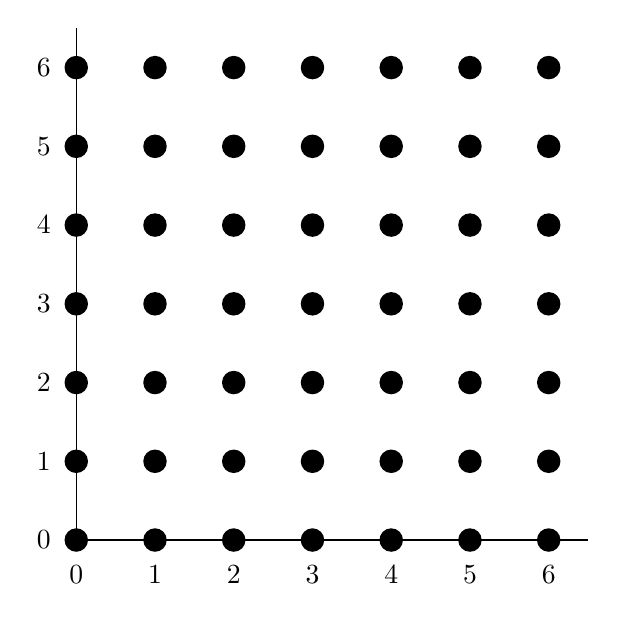
\begin{tikzpicture}[scale=1]
        \foreach \x in {0,...,6}
            {
                \foreach \y in {0,...,6}
                    {
                        \node at (\x, \y)[circle,fill,inner sep=3pt]{};
                    }
                \node[left] at (-0.2, \x){$\x$};
                \node[below] at (\x, -0.2){$\x$};
            }

        \draw (0.0, 0.0) -- (6.5, 0.0);
        \draw (0.0, 0.0) -- (0.0, 6.5);
    \end{tikzpicture}
\end{center}
这个平面上的``点阵''被称为\emph{格 (Lattice)}。一个有趣的问题是:在格中,给定任意一点,从原点 $(0, 0)$ 到该点有多少条路径?具体来说,我们将\textbf{格路径}定义为从 $(0, 0)$ 到特定点的路径,且每一步只能\emph{向右}或\emph{向上}移动。以下定义详细说明了这一概念:

\begin{definition}
    设 $(x,y) \in (\mathbb{N} \cup \{0\})^2$。到 $(x, y)$ 的\dotuline{格路径}是二维格中的一个有序格点元组,其中元组的第一个元素为 $(0, 0)$,最后一个元素为 $(x, y)$,且每个点与前一个点相比,恰好有一个坐标增加一个单位。

    更严格地说,给定 $(x, y)$,格路径是一个 $n \in \mathbb{N}$ 元组 $(P_1, P_2, \dots, P_n)$,其中每个 $P_i = (x_i, y_i)$ 是格中的一个点,且满足:
    \[\forall i \in [n - 1] \centerdot (x_{i+1}, y_{i+1}) = (x_i + 1, y_i) \lor (x_{i+1}, y_{i+1}) = (x_i, y_i + 1)\]
    同时,$(x_1, y_1) = (0, 0)$ 且 $(x_n, y_n) = (x, y)$。

    也就是说,格路径是从 $(0, 0)$ 到 $(x, y)$ 的一系列格点,其中每一步只允许向右或向上移动一个单位。
\end{definition}

\begin{example}
    考虑二维格点 $(2,4)$。如下图所示,我们展示了从原点到 $(2,4)$ 的几条格路径。

    \begin{center}
        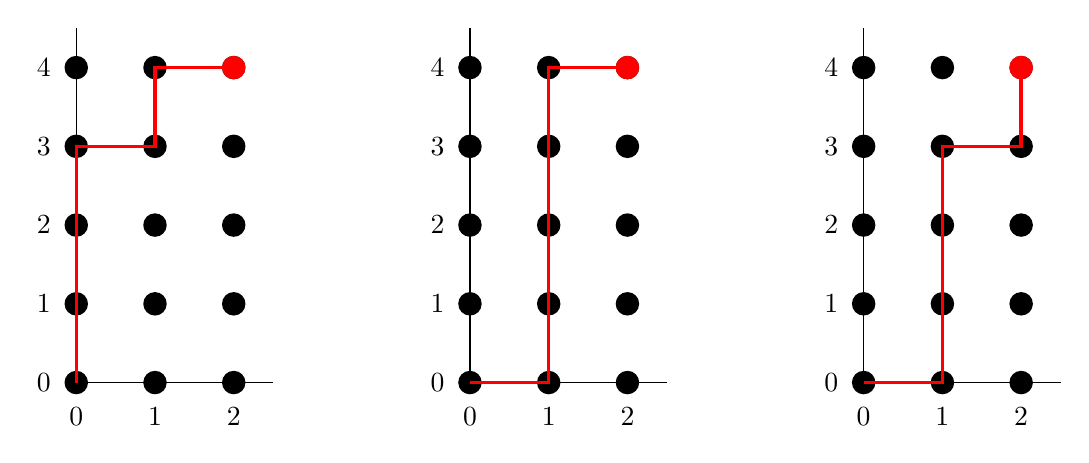
\begin{tikzpicture}[scale=1]
            \foreach \n in {0,5,10}
                {
                    \foreach \x in {0,...,2}
                        {
                            \foreach \y in {0,...,4}
                            \node at (\x+\n, \y)[circle,fill,inner sep=3pt]{};

                            \node[below] at (\x+\n, -0.2){$\x$};
                        }
                    \foreach \y in {0,...,4}
                    \node[left] at (\n-0.2, \y){$\y$};

                    \draw (\n, 0.0) -- (2.5+\n, 0.0);
                    \draw (\n, 0.0) -- (\n, 4.5);
                    \node[red] at (\n+2.0, 4.0)[circle,fill,inner sep=3pt]{};
                }
            \draw[red, very thick] (0.0, 0.0) -- (0.0, 3.0) -- (1.0, 3.0) -- (1.0, 4.0) -- (2.0, 4.0);
            \draw[red, very thick] (5.0, 0.0) -- (6.0, 0.0) -- (6.0, 4.0) -- (7.0, 4.0);
            \draw[red, very thick] (10.0, 0.0) -- (11.0, 0.0) -- (11.0, 3.0) -- (12.0, 3.0) -- (12.0, 4.0);
        \end{tikzpicture}
    \end{center}

    我们的问题是:

    \begin{quotation}
        给定 $(a,b) \in (\mathbb{N} \cup \{0\})^2$,从原点到 $(a, b)$ 有多少条\emph{不同的}格路径?
    \end{quotation}

    为了回答这个问题,我们先来看一个简单的例子,使用较小的数值以便枚举所有路径。假设我们考虑从 $(0, 0)$ 到 $(2, 2)$ 的格路径:

    \begin{center}
        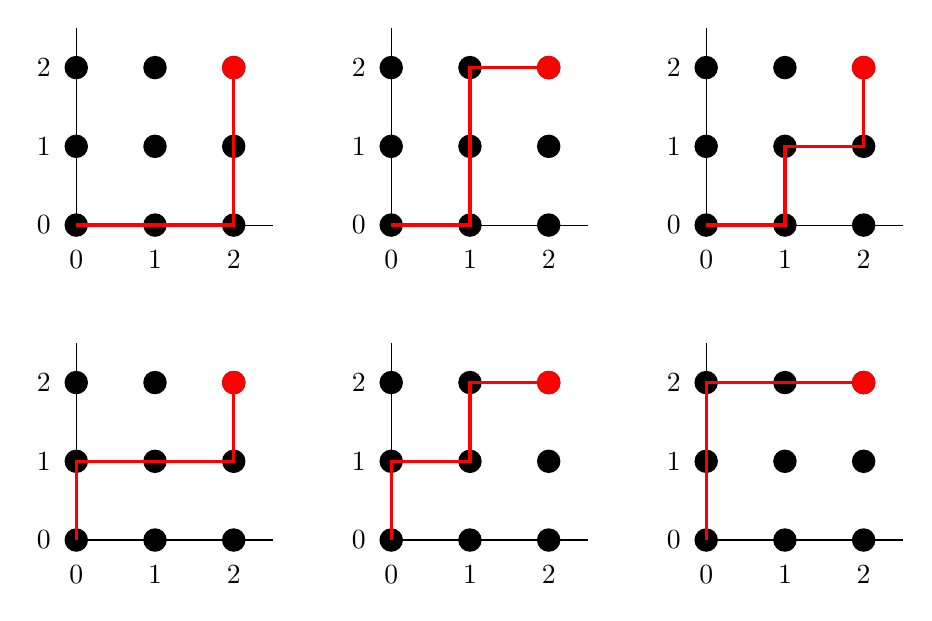
\begin{tikzpicture}[scale=1]
            \foreach \m in {0, 4}
                {
                    \foreach \n in {0, 4, 8}
                        {
                            \foreach \x in {0,...,2}
                                {
                                    \foreach \y in {0,...,2}
                                    \node at (\x+\n, \y+\m)[circle,fill,inner sep=3pt]{};

                                    \node[left] at (\n-0.2, \x+\m){$\x$};
                                    \node[below] at (\x+\n, \m-0.2){$\x$};
                                }

                            \draw (\n, \m) -- (2.5+\n, \m);
                            \draw (\n, \m) -- (\n, 2.5+\m);
                            \node[red] at (\n+2.0, \m+2.0)[circle,fill,inner sep=3pt]{};
                        }
                }
            \draw[red, very thick] (0.0, 0.0) -- (0.0, 1.0) -- (2.0, 1.0) -- (2.0, 2.0);
            \draw[red, very thick] (4.0, 0.0) -- (4.0, 1.0) -- (5.0, 1.0) -- (5.0, 2.0) -- (6.0, 2.0);
            \draw[red, very thick] (8.0, 0.0) -- (8.0, 2.0) -- (10.0, 2.0);

            \draw[red, very thick] (0.0, 4.0) -- (2.0, 4.0) -- (2.0, 6.0);
            \draw[red, very thick] (4.0, 4.0) -- (5.0, 4.0) -- (5.0, 6.0) -- (6.0, 6.0);
            \draw[red, very thick] (8.0, 4.0) -- (9.0, 4.0) -- (9.0, 5.0) -- (10.0, 5.0) -- (10.0, 6.0);
        \end{tikzpicture}
    \end{center}

    我们如何用\emph{组合的}方式来表示格路径呢?也就是说,怎样表示才能方便我们计数这些路径?回想格路径的定义:在构建路径的每一步中,每次``移动''都必须向右或向上。因此,用符号表示每次``向右''和``向上''移动是有意义的。然后,我们只需要计算有多少种由``向右''和``向上''移动组成的序列能带我们到达目标点 $(x, y)$。

    这其实很简单!平面上的点 $(x, y)$ 有什么特征呢?它位于 $(0,0)$ 的右边 $x$ 个单位、上方 $y$ 个单位。因此,无论路径如何,从 $(0,0)$ 到 $(x,y)$ 必须恰好有 $x$ 次向右移动和 $y$ 次向上移动。回顾上面到 $(2, 2)$ 的 $6$ 条格路径。想象沿着路径,从 $(0, 0)$ 开始,在每一步根据移动方向写下 $R$(右)或 $U$(上)。这样就得到了以下 $6$ 个由 $R$ 和 $U$ 组成的序列:
    \[RRUU \:,\: RUUR \:,\: RURU \:,\: URRU \:,\: URUR \:,\: UURR\]

    这些序列有什么共同特征?每个序列都有 $2$ 个 $R$ 和 $2$ 个 $U$,并且总长度为 $4$,因为从 $(0,0)$ 到 $(2,2)$ 需要 $2+2=4$ 步。这类似于一个受限的字母表/单词问题:我们希望从字母表 $\{R,U\}$ 中组成长度为 $4$ 的单词,其中 $R$ 和 $U$ 都恰好出现 $2$ 次!

    通常情况下,我们知道从 $(0,0)$ 到 $(x,y)$ 的任意格路径可以表示为一个长度为 $x+y$ 的序列,其中恰好包含 $x$ 个 $R$ 和 $y$ 个 $U$。为了确定这样的序列有多少个,我们可以分两步进行:
    \begin{enumerate}
        \item 从 $x + y$ 个空位中选择 $x$ 个填充 $R$:有 ${x+y \choose x}$ 种方式;
        \item 剩下的 $(x + y) - x = y$ 个空位填充 $U$:只有 $1$ 种确定的填充方式。
    \end{enumerate}
    因此,我们得到如下结论。

    \begin{proposition}
        对于每个 $(x,y) \in (\mathbb{N} \cup \{0\})^2$,从 $(0,0)$ 到 $(x,y)$ 恰有 ${x+y \choose x}$ 条格路径。
    \end{proposition}

    我们将在练习中探索格路径的更多应用和性质。目前,我们想强调格路径的存在及其与序列和选择之间的关系。但这里还有一个有趣的观察:为什么我们选择计算长度为 $x+y$ 的序列中恰好有 $x$ 个 $R$ 的数量?如果计算恰好有 $y$ 个 $U$ 的数量,会有什么不同吗?思考一下:每条到 $(x, y)$ 的格路径必须恰好有 $x$ 个 $R$ 和 $y$ 个 $U$,因此确保其中一个条件成立自然保证了另一个条件。于是,我们得到以下结论:

    \begin{proposition}
        对于每个 $(x,y) \in (\mathbb{N} \cup \{0\})^2$,从 $(0,0)$ 到 $(x,y)$ 恰有 ${x+y \choose y}$ 条格路径。
    \end{proposition}
    这不仅证明了如下事实
    \[{x+y \choose x} = {x+y \choose y}\]
    而且也引出了一种有用的证明策略:\textbf{两法计数}。我们确定了一组对象(从 $(0, 0)$ 到 $(x, y)$ 的格路径集合),并给出了两种\emph{不同的}计数方法。每种方法得到了该集合基数的不同表达式,因此这两个表达式必然相等。这个例子展示了两法计数的核心思想,我们将在下一节进一步探讨这一技术及其应用。
\end{example}